%! TEX root = asd-beamer.tex
\documentclass[asd-beamer.tex]{subfiles}

\begin{document}
	
\section{Test ipotesi Bayesiano}

\begin{frame}{MAP Test}
Choose hypothesis with maximum a posteriori probability: $\prob{(H_i|Y=y)}$
\end{frame}

\section{Test di ipotesi frequentista}\linkdest{testfreq}

%\begin{frame}[allowframebreaks]{List of things}
%\printbibliography[keyword={inference},heading=beamer]
%\printbibliography[keyword={\mybibcat},heading=beamer]
%\listofkeywords
%\end{frame}

\subsection{Accepting or rejecting hypothesis}\linkdest{Htest}
	
\begin{frame}{Formulazione matematica test tra ipotesi alternative}\frameintoc
\begin{block}{Partizione di X in \keyword{regione di accettanza/critica}}
Decisione basata su valore di RV X la cui pdf $P_{\theta}$ che appartiene a una classe di pdf $\mathcal{P}=\{P_{\theta}, \theta\in\Omega\}$:  $\mathcal{P}=H\cup K$ denotano classi mutualmente esclusive di pdf rel a 2 ipotesi sullo spazio dei parametri con $\Omega=\Omega_H\cup\Omega_K$ (se il parametro \'e noto sappiamo con certezza se vera/falsa). Se indico $d_0/d_1$ la decisione di accettare/rifiutare assegno ogni $x\in X$ a regioni complementari $S_0/S_1$ regione di accettanza/critica.
\end{block}
\begin{block}{Test function and power}
Test function $\psi(X)$ stands for prob. with wich null hypothesis is rejected when $X=x$ is observed, power $Q(\theta)=\E_{\theta}[\psi(X)]$.
%Fissato $\cl=1-\alpha$ impongo la condizione
%P_{\theta}[\delta(X)=d_1]=
%\[P_{\theta}[X\in S_1]\leq\alpha,\quad \forall\theta\in\Omega_H\]
%minimizzo $P_{\theta}[\delta(X)=d_0]$ $\forall\theta\in\Omega_K$ equiv. to maximize
%P_{\theta}[\delta(X)=d_1]=
%\[1-\beta=P_{\theta}[X\in S_1], \forall\theta\in\Omega_K\]
%Di solito la condizione precedente implica size of test $\sup_{\Omega_H}{P_{\theta}[X\in S_1]}=\alpha$.
\end{block}
\end{frame}

\begin{frame}{Errori: tipo I (rifiuto ipotesi vera), tipo II (accetto ipotesi falsa)}
\begin{block}{ \keyword{Prob. Errore tipo I $\alpha$}}
	scarto $H_0$ quando \'e vera: probabilit\'a di errore I $\alpha=\prob{(x\in S_1|H_0)}=\prob_0{(x\in S_1)}$: \keyword{livello di significativit\'a}. \keyword{Livello di confidenza} $1-\alpha=\prob{(x\in S_0|H_0)}$
\end{block}
\begin{block}{\keyword{Prob. Errore tipo II $\beta$}}
	probabilit\'a di accettare erroneamente $H_0$ (falso negativo, contaminazione), $\prob{(x\in S_0|\non{H_0})}=\beta$. Potenza del test $1-\beta=\prob{(x\in S_1|H_1)}$ \'e la capacit\'a di distinguere ipotesi diverse da $H_0$ 
\end{block}
\end{frame}

\begin{frame}{Symmetry between $\alpha$ and $\beta$}
Unrealistic in experimental situation to keep $\alpha$ constant:$\alpha=p(\theta_0)$ $\beta=p(\theta_1)$ as function of $\alpha$, dotted line $\alpha=1-\beta$ below which tests are unbiased
\begin{figure}[!ht]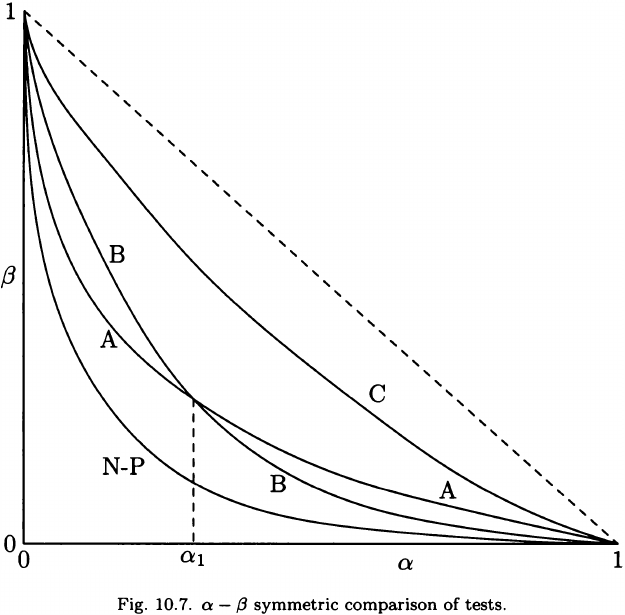
\includegraphics[trim={0cm 0cm 0 0},clip, keepaspectratio,width=0.5\textwidth]{figures/james/test/testabsym}\label{fig:testabsym}\end{figure}
\end{frame}

\begin{frame}{Comparison of tests: power}
Ipotesi semplici: $H_0: \theta=\theta_0$, $H_1: \theta=\theta_1$. Power $1-\beta=p(\theta_1)$.
Ipotesi composte: $p(\theta)=1-\beta(\theta)$.
\begin{columns}[T]
\begin{column}{0.4\textwidth}
\begin{figure}[!ht]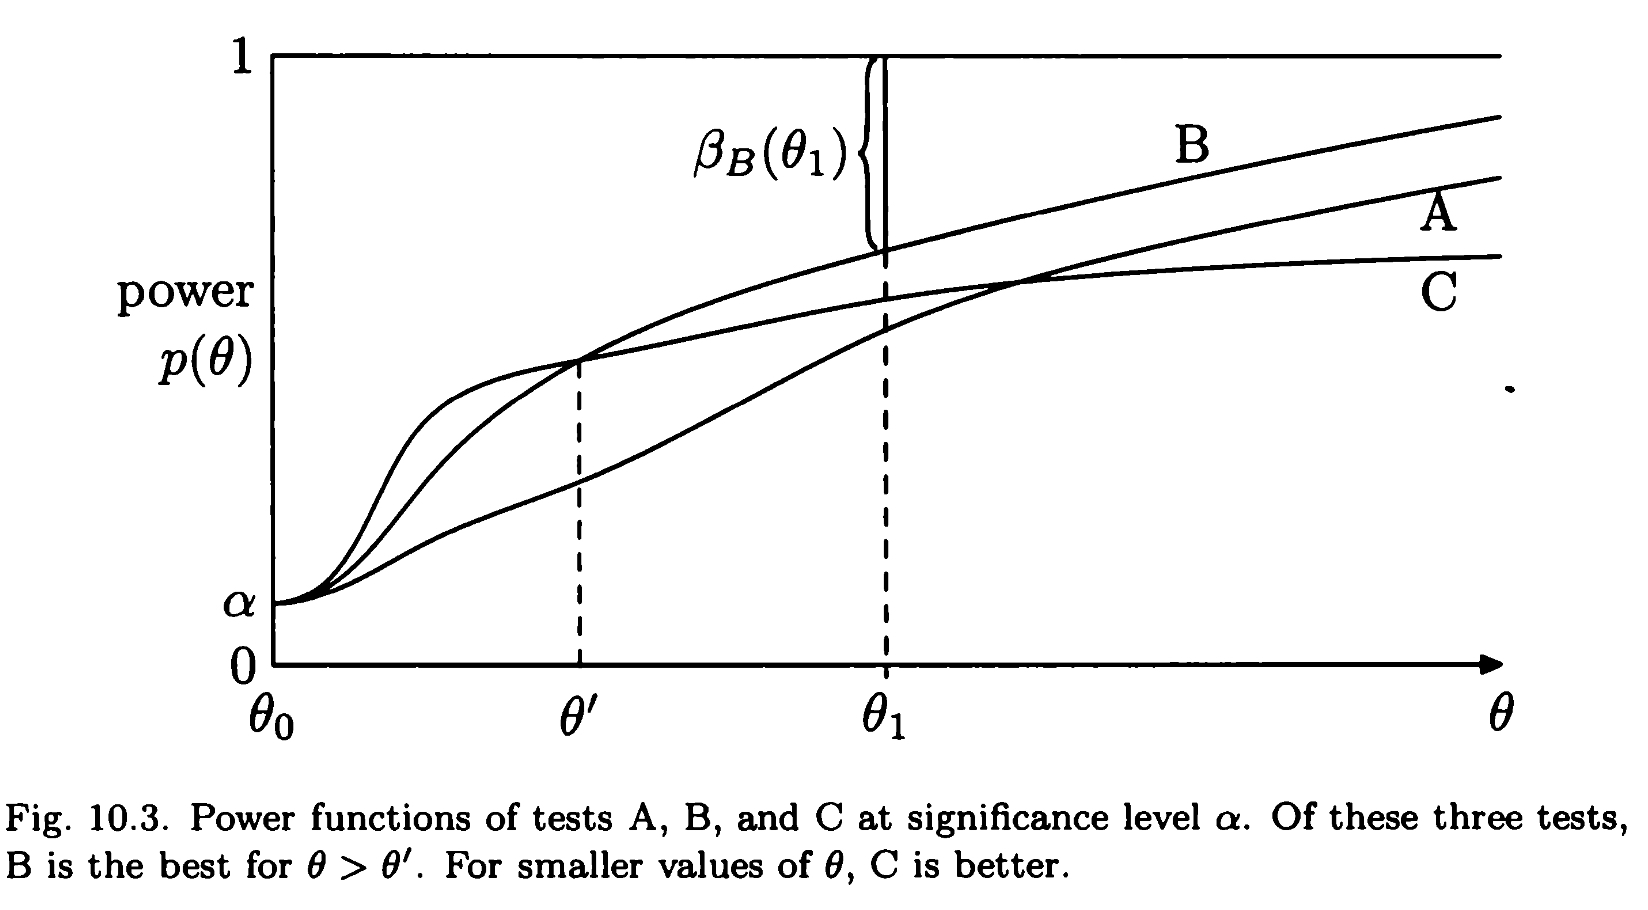
\includegraphics[trim={0cm 0cm 0 0},clip, keepaspectratio,width=0.99\textwidth]{figures/james/test/mostpower}\label{fig:mostpower}
\end{figure}
\end{column}
\begin{column}{0.6\textwidth}
\begin{block}{Ottimizzazione: power maggiore possibile.}
	UMP test: power maggiore uguale a qualunque test per tutte le ipotesi: esiste?
\end{block}
\end{column}
\end{columns}
\begin{block}{Per ipotesi composte non esiste test UMP generale}
	One family pdf $f(\vec{X},\theta)$: MP test of $H_0$ per $\theta<\theta_0$, $H_1$ per $\theta>\theta_1$ in general depends on $\theta_1$ thus not uniform
\end{block}
\end{frame}

\begin{frame}{Consistenza e bias}
\begin{columns}[T]
	\begin{column}{0.5\textwidth}
\begin{itemize}
	\item \keyword{Consistenza}: $\lim_{N\to\infty}\prob{(\vec{X}\in  S_1|H_1)}=1$ non \'e detto che sia uniforme.
	\item \keyword{unbiasedness} $\pow{}=1-\beta\geq\alpha, \forall i$, T consistente \'e asintoticamente unbiased.
\end{itemize}
	\end{column}
	\begin{column}{0.5\textwidth}
\begin{figure}[!ht]\begin{subfigure}[b]{0.99\textwidth}
		\centering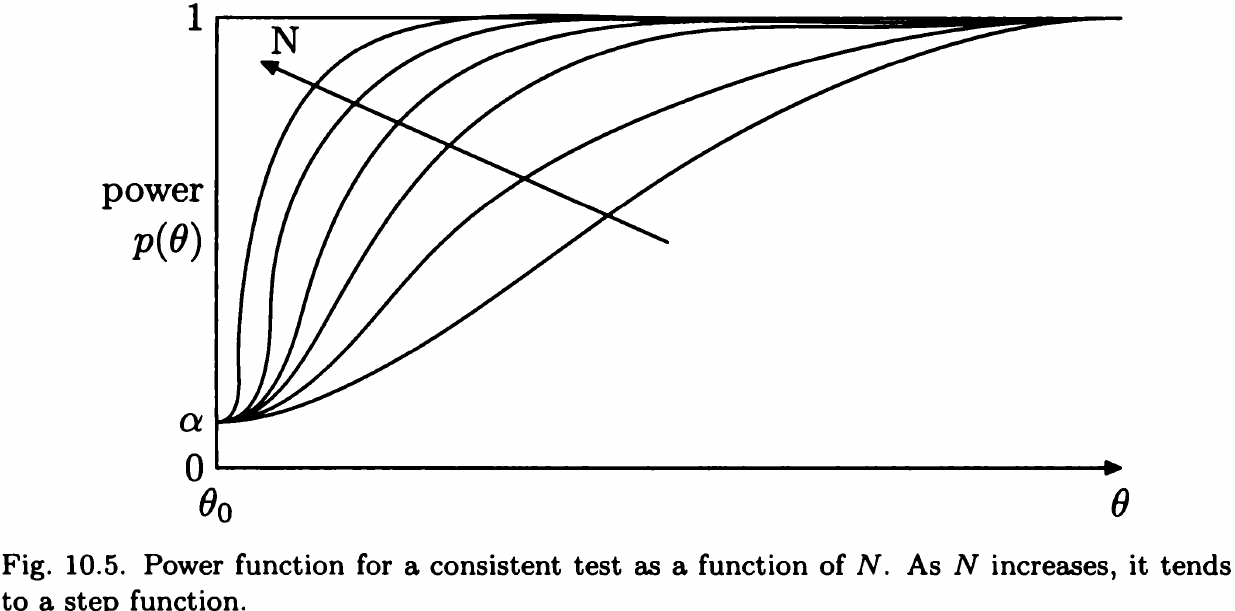
\includegraphics[trim={0cm 0 0 0},clip, width=0.99\textwidth]{figures/james/test/powerconsistent}\label{fig:powerconsistent}\end{subfigure}~
	\begin{subfigure}[b]{0.99\textwidth}\centering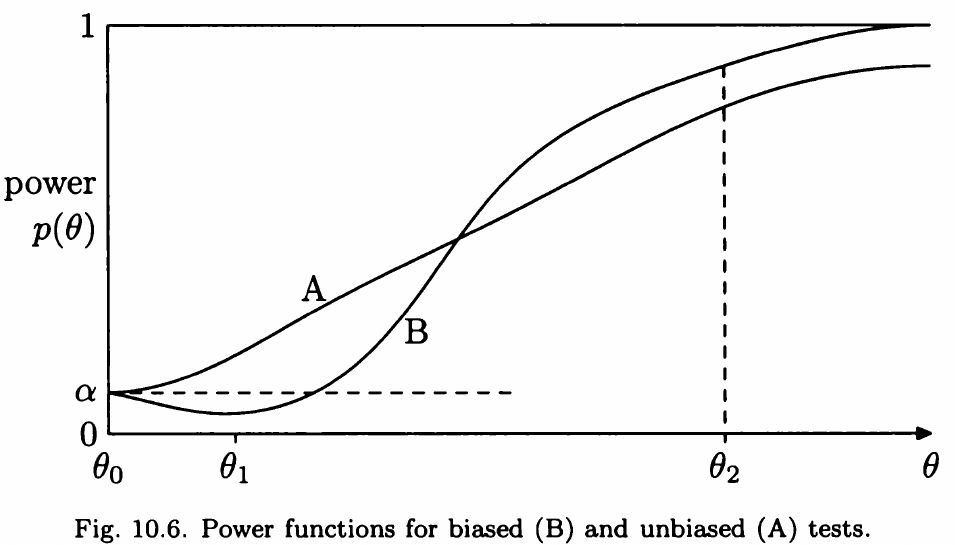
\includegraphics[trim={0cm 0 0 0},clip,width=0.99\textwidth]{figures/james/test/biasedtest}\label{fig:biasedtest}\end{subfigure}\end{figure} 
Test B can't distinguish between $\theta_0$, $\theta_1$.
	\end{column}
\end{columns}
\end{frame}

\begin{frame}{Properties of tests}
\begin{block}{Test Unbiased}
Hypothesis $H: \theta\in\Omega_H$ vs $K:\theta\in\Omega_K$. Unbiasedness: for no alternatives in K probability of rejection is less then size of test
\begin{align*}
&\pow{}=\E_{\theta}{[\phi(X)]}\leq\alpha\tag{$\theta\in\Omega_H$}\\
&\pow{}=\E_{\theta}{[\phi(X)]}\geq\alpha\tag{$\theta\in\Omega_K$}
\end{align*}
\end{block}
\begin{block}{Invarince and symmetry}
$X\in f(x;\theta)$ con $\theta\in\Omega$; g trasformazione 1-1 dello spazio campionario in se: $gX$ denota RV con valore $gx$ quando $X=x$ con pdf $f(x;\theta')$ cos\'i definisco $\overline{g}\theta=\theta'\in\Omega$. Lo spazio dei parametri \'e invariqante sotto g se $\overline{g}\Omega=\Omega$.
\keyword{Invariant test under G:} $\phi(gx)=\phi(x)$ per ogni $x\in X$ e $g\in G$ inoltre $\overline{g}\Omega_H=\Omega_H$ e lo stesso $\Omega_K$
\end{block}
\end{frame}

\subsection{Ipotesi semplici}\linkdest{Hsimple}

\begin{frame}{Testing simple hypothesis}
\begin{block}{Test: funzione dallo spazio delle osservabili in H.}
	Un'ipotesi \'e un'affermazione sui parametri che caratterizzano lo stato della natura; se l'ipotesi non \'e sufficienta a determinare distribuzione di probabilit\'a della nostra osservabile l'ipotesi \'e composta: se ipotesi da falsificare \'e non esistenza higgs ($m=0$) semplice, ma alternativa \'e composta da $m>0$
\end{block}
\begin{block}{Ratio statistics}
Discrete distribution $P_i[X=x]=P_i(x)$: optimum test is defined as critical region S satisfying
\begin{columns}[T]
\begin{column}{0.5\textwidth}
\begin{align*}
&\sum_{x\in S}P_0(x)\leq\alpha\\
&\sum_{x\in S}P_1(x)=\max{}
\end{align*}
\end{column}
\begin{column}{0.5\textwidth}
Most valuable points x are those with highest \[r(x)=\frac{P_1(x)}{P_0(x)}\]
\end{column}
\end{columns}
S is the set of x points $x: r(x)>c$ where c is determined by \[P_0[X\in S]=\sum_{x: r(x)>c}P_0(x)=\alpha\]
\end{block}
\end{frame}

\begin{frame}{Lemma di Neyman-Pearson (Test di NP)}\frameintoc\linkdest{NPtest}
\begin{block}{Statistica di un test}
Posso esprimere un test in funzione di una statistica: $T(\vec{x})=T(t(\vec{x}))$ (nel caso del lemma NP la statistica \'e il LR). 
\end{block}
\begin{block}{Test NP}
%Lo spazio dei parametri \'e costituito da $\theta_0$, $\theta_1$: l'MP test \'e quello che mi da come regione critica gli x tali che $\frac{\prob_0{(x)}}{\prob_1{(x)}}<q(\alpha)$, $q$ \'e determinato da condizione $\prob{(C|H_0)}\leq\alpha$ (LR), questo \'e il test di massimo power.
RV $\vec{X}$: pdf $f_N(\vec{X}|\theta)$, lo spazio dei parametri \'e $\theta_0,\theta_1$. Cerco la regione critica $w_{\alpha}$ che massimizza power $1-\beta$ (dato $\alpha$):
\begin{align*}
&\int_{w_{\alpha}}f_N(\vec{X}|\theta_0)\,dX=\alpha\\
&\int_{w_{\alpha}}f_N(\vec{X}|\theta_1)\,dX=1-\beta\\
&=\int_{w_{\alpha}}\frac{f_N(\vec{X}|\theta_1)}{f_N(\vec{X}|\theta_0)}f_N(\vec{X}|\theta_0)\,dX=\E_{w_{\alpha}}{[\frac{f_N(\vec{X}|\theta_1)}{f_N(\vec{X}|\theta_0)}|\theta_0]}\\
&\Rightarrow l_N(\vec{X},\theta_0,\theta_1)=\frac{f_N(\vec{X}|\theta_1)}{f_N(\vec{X}|\theta_0)}\geq c_{\alpha}: H_1\ (\leq c_{\alpha}: H_0)
\end{align*}
\end{block}
\end{frame}

\begin{wordonframe}{Dimostrazione lemma Neyman-Pearson}
Per ogni test alternativo $T'$ prendo $\alpha'\leq\alpha_{NP}$ allora $\beta'\geq\beta_{NP}$ ($\pow'\leq\pow_{NP}$, probabilit\'a errore tipo II \'e maggiore), dimostro $\beta'-\beta\geq0$ cio\'e $\prob{(\overline{C}'|H_1)}-\prob{(\overline{C}|H_1)}$:
\begin{align*}
&\prob{(C|H_1)}-\prob{(C'|H_1)}=\prob{(C\cap|H_1)}+\prob{(C\cap\overline{C}'|H_1)}-\prob{(C\cap C'|H_1)}\\
&-\prob{(C'\cap\overline{C}|H_1)}=\prob{(C\cap\overline{C}'|H_1)}-\prob{(C'\cap\overline{C}|H_1)}\\
&\prob{(C\cap C'|H_1)}=\int_{C\cap C'}\prob_1{(x)}\,dx\geq\int_{C\cap \overline{C}'}\frac{\prob_0{(x)}}{q}\,dx=\frac{1}{q}\prob{(C\cap\overline{C}'|H_0)}
\end{align*}
dove si \'e usata la relazione di de morgan per complementare di intersezioni e la disuguaglianza del lemma-NP
\end{wordonframe}

\subsection{Ipotesi composte}\linkdest{Hcomposite}

\begin{frame}{Monotone Likelihood property}\frameintoc
\begin{block}{\keyword{Monotone LR}}
Real parameter family of density $p_{\theta}(x)$ is said to have Monotone LR if exists statistics $T(x)$ for $\theta<\theta'$ le distribuzioni sono distinte e $\frac{P_{\theta'}(x)}{P_{\theta}(x)}$ \'e funzione non-decrescente/non-crescente di $T(x)$: this results in placing rejection region in upper/lower tail of the distribution of test statistics under $H_0$
\begin{columns}[T]
	\begin{column}{0.5\textwidth}
		Non-decreasing LR:
		\begin{align*}
		&\psi(X)=\lbt{1:\ T(X)>k}{0:\ T(X)<k}
		\end{align*}
	\end{column}
	\begin{column}{0.5\textwidth}
		Non-increasing LR:
		\begin{align*}
		&\psi(X)=\lbt{1:\ T(X)<k}{0:\ T(X)>k}
		\end{align*}
	\end{column}
\end{columns}
\end{block}
\begin{block}{One param exponential family}
Sia $T(x)$ stat sufficiente per parametro $\theta$ e 
\begin{equation*}
g(t;\theta)=a(\theta)c(t)\exp{tb(\theta)}
\end{equation*}
con t del dominio di T. Le funzioni di questa famiglia godono del Monotone Likelihood Ratio property
\end{block}
\end{frame}

\begin{frame}{Test UMP unilaterale per famiglia esponenziale}\linkdest{UMPtestexp}
%Karlin-Rubin theorem
$X_1,\ldots,X_N$ N iid: pdf della forma $\prob{(x,\mu)}=F(x)G(\mu)\Exp{[A(x)B(\mu)]}$ e $B(\mu)$ (monotona):

UMP test (one-sided) per distinguere $H_0: \mu=\mu_0$, $H_{\mu}: \mu>\mu_0$; applico NP per $\mu_0$ e $\mu$, MP test ha la forma

\[\frac{F^N(x)G^N(\overline{\mu})}{F^N(x)G^N(\overline{\mu}_0)}\Exp{[\sum_iA(x_i)](B(\overline{\mu})-B(\overline{\mu}_0))}\gtrless c_{\alpha}\]
$F,G>0$.
Se il likelihood ratio \'e funzione monotona (non-decrescente) di una statistica $T(\vec{X})=\sum_iA(x_i)$ e scelgo $\alpha$ e $k_{\alpha}$ tali che $\prob{[\lr{(T(x))}\geq c_{\alpha}]}=\alpha$  allora la regione critica per un test UMP unilaterale $H_0$ vs $H_1$ \'e $C=\{x:T(x)\geq k_{\alpha}\}$.

\cite[5]{lrtmptumpt}; \cite[445]{inferencemukhopadhyay2000}; \cite[sec 3.6]{lehmann2006testing}
\end{frame}

\begin{frame}{Test UMP parametro non contenuto nell'intervallo vs contenuto (ma non viceversa)}

\cite[269]{james2006statistical}\cite[sec 3.7]{lehmann2006testing}
\end{frame}

\begin{wordonframe}{No UMP test for two-sided hypothesis}
%insert-fig 10.9: oneone2sides
$1+$ \'e il power per UMP test per $\theta>\theta_0$, $1-$ \'e il power per UMP test per $\theta<\theta_0$: if the size of one sided tests is $\frac{\alpha}{2}$ that of two-sided (sum of the two one-sided) is $\alpha$
\begin{figure}[!ht]
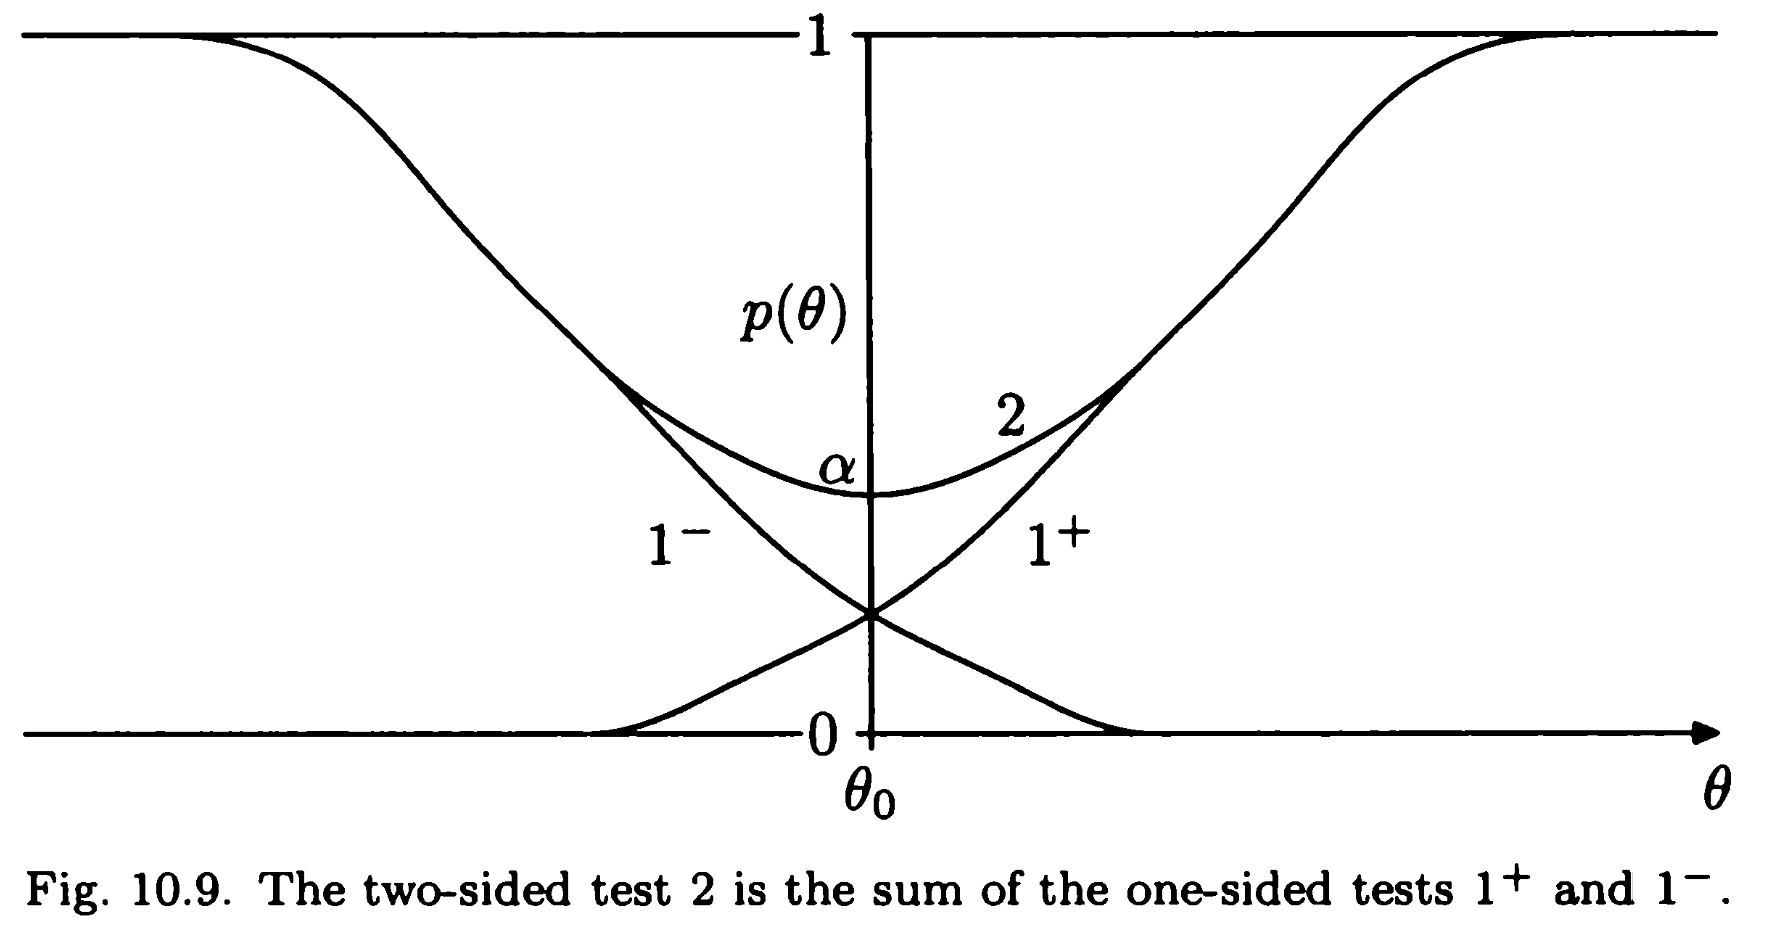
\includegraphics[trim={0cm 0cm 0 0},clip, keepaspectratio,width=0.5\textwidth]{figures/james/test/oneone2sided}
\label{fig:oneone2sided}
\end{figure}

\end{wordonframe}

\begin{frame}{Locally most powerfull (LMP) tests}\linkdest{LMP}
(LMP) (Se non esiste UMP test) Se ho bisogno di massima sensibilit\'a vicino alla soglia: $1-\beta$ grande nelle vicinanze di $\theta_0$: $H_0$: $\theta=\theta_0$, $H_1$: $\theta=\theta_0+\Delta$, quindi $\ln{L(\vec{X},\theta_1)}\approx\ln{L(\vec{X},\theta_0)}+\Delta\PDy{\theta}{\ln{L}}|_{\theta_0}$.
Applico NP a $H_0$ vs $H_1$:
\begin{align*}
&\ln{L(\vec{X},\theta_1)}-\ln{L(\vec{X},\theta_0)}\gtrless c_{\alpha} \Rightarrow \PDy{\theta}{\ln{L}}\gtrless q_{\alpha}\\
&\E{[\PDy{\theta}{\ln{L}}|_{\theta_0}]}=0,\ \E{[(\PDy{\theta}{\ln{L}})^2]}=NI
\end{align*}
score \'e asintoticamente normale Test: $\PDy{\theta}{\ln{L}}|_{\theta_0}\gtrless\lambda_{?1-\alpha}\sqrt{NI}$.
\end{frame}

\begin{frame}{Likelihood ratio test (LRT)}\frameintoc\linkdest{LRT}
Sia $H_0: \vec{\theta}\in\nu$, $H_0: \vec{\theta}\in\overline{\nu}$
\begin{columns}[T]
\begin{column}{0.4\textwidth}
\begin{align*}
&H_0: \theta_i=\theta_{i0}, i=1,\ldots,r\\
&\theta_j, j=1,\ldots,s\\
\end{align*}
\end{column}
\begin{column}{0.6\textwidth}
\begin{align*}
&H_1: \theta_i\neq\theta_{i0}, i=1,\ldots,r\\
&\theta_j, j=1,\ldots,s
\end{align*}
\end{column}
\end{columns}
\begin{block}{test statistic maximum likelihood ratio}
\begin{align*}
&\lambda=\frac{\max_{\vec{\theta}\in\nu}L(\vec{X},\theta)}{\max_{\vec{\theta}\in\overline{\nu}}L(\vec{X},\theta)}=\frac{\max_{\vec{\theta}_s}L(\vec{X}|\vec{\theta}_{r0},\vec{\theta}_s)}{\max_{\vec{\theta}_r, \vec{\theta}_s}L(\vec{X}|\vec{\theta}_r,\vec{\theta}_s)}
\end{align*}
Asymptotic pdf of $\hat{\theta}=(\hat{\theta}_r,\hat{\theta}_s)$ is $(r+s)$-D Normal with covariance matrix $\invers{I}$
\end{block}
\end{frame}

\begin{frame}{LR test: critical region, significance level and power for continuus families of Hypotheses}
	%$\alpha=\sup{\prob{(\lambda(\vec{X})\leq k;\theta\in\theta_0)}}$.
	Se $H_0$ impone r vincoli sugli $r+s$ parametri di $H_0, H_1$: $\forall\theta\in H_0$ $-2\log{\lambda}\to\chi^2_{r}$, $\forall\theta\in H_1$ $-2\log{\lambda}\to\chi^2_{r}$ non centrale con parametro $K_1=(\vec{\theta}_r-\vec{\theta}_{r0})^TI_r(\vec{\theta}_r-\vec{\theta}_{r0})$.
	Regione critica: $-2\ln{\lambda}>\chi^2_{\alpha}(r)$, power:
	\begin{equation*}
	p=1-\beta=\int_{\chi_{\alpha}^2(r)}^{\infty}dF_1[\chi^2(r,K_1)]\approx\int_{(\frac{r+K_1}{r+2K_1})\chi^2_{\alpha}(r)}^{\infty}dF_2[\chi^2(r+\frac{K_1^2}{r+2K_1})]
	\end{equation*}
\end{frame}

\begin{wordonframe}{LRT: }
\begin{block}{Likelihood asymptotic expression}
Asymptotically MLE $\hat{\theta}$ attains MVB:
\begin{align*}
&L(\vec{X}|\theta)=-\E{[\PtwoDy{\theta}{\ln{L}}]}(\hat{\theta}-\theta)\\
&L(\vec{X},\vec{\theta})=L(\vec{X},\vec{\theta}_r,\vec{\theta}_s)\propto\Exp{[-\frac{1}{2}(\hat{\theta}-\vec{\theta})^TI(\hat{\theta}-\vec{\theta})]}\\
&\lambda=\frac{L(\vec{X}|\theta_r,\hat{\theta}_s)}{L(\vec{X}|\hat{\theta_r},\hat{\theta}_s)}=\Exp{[-\frac{1}{2}(\hat{\theta}_r-\theta_{r0})^TI_r(\hat{\theta}_r-\theta_{r0})]}
\end{align*}
\end{block}
\begin{block}{Espansione in $\hat{\theta}-\theta_0$ per $\theta=\theta_0$}
	Usually the critical region is determined via asymptotic pdf of LR:
	$l(\theta_0)=-\log{L}=l(\hat{\theta})+\frac{1}{2}l''(\hat{\theta})(\hat{\theta}-\theta_0)^2$ $L(\vec{X}|\vec{\theta})\propto\exp{-\frac{1}{2}\E{(\PtwoDy{\theta}{\ln{L}})}(\hat{\theta}-\theta)^2}=\exp{-\frac{1}{2}(\hat{\theta}-\theta)^TI(\hat{\theta}-\theta)}$ (pdf asintoticamente normale con matrice covarianza $\invers{I}$). Quindi $I(\theta_0)(\hat{\theta}-\theta)^2\xrightarrow{D}\chi_1^2$.
\end{block}
\begin{block}{Asymptotic properties of MLE}

\end{block}
\end{wordonframe}

\begin{wordonframe}{Test of some theories with different dof}
%insert-fig 10.10
Maximum likelihood ratio for A vs generale case: $\lambda_a=\frac{L(0)}{L(d)}$, if hypothesis A is true $-2\ln{\lambda_a}$ is distributed asymptotically as $\chi^2(2)$; to test B vs general case ml ratio is $-2\ln{\lambda_a}$, distributed asymptotically as $\chi^2(1)$.
\end{wordonframe}

\begin{wordonframe}{Is data normally distributed (unknown variance)}
$X_1,,X_N$ iid $N(\mu,\sigma^2)$, $H_0: \mu=0,\sigma^2$, $H_1: \mu\neq0,\sigma^2$. Likelihood function is: 
\begin{equation*}
L(\mu,\sigma^2)=\frac{1}{(2\pi)\expy{N/2}\sigma^N}\exp{-\frac{1}{2}\sum^N\frac{(X_i-\mu)^2}{\sigma^2}}
\end{equation*}
Maximum likelihood estimators:
\begin{align*}
&H_0: \hat{\sigma}^2=\frac{1}{N}\sum_iX_i^2\\
&\max_{\sigma^2}L(0,\sigma)=\frac{\exp{-N/2}}{(2\pi)\expy{N/2}(\sum_iX_i/N)\expy{N/2}}\\
&H_1: \hat{\mu}=\exv{X},\ S^2=\frac{1}{N}\sum^N(X_i-\exv{X})^2\\
&\max_{\sigma^2}L(0,\sigma)=\frac{\exp{-N/2}}{(2\pi)\expy{N/2}(\sum_i(X_i-\exv{X})^2/N)\expy{N/2}}\\
\end{align*}
Likelihood ratio:
\begin{align*}
&\lambda=(\frac{\sum^N(X_i-\exv{X})^2}{\sum_iX_i^2})\expy{N/2}\\
&\lambda\expy{2/N}=\frac{1}{1+\frac{t^2}{N-1}}\\
&t=\frac{\sqrt{N}\exv{X}}{\sqrt{\frac{1}{N-1}}\sum(X_i-\exv{X})^2}=\sqrt{N}\frac{\exv{X}}{s}
\end{align*}
Test based on $\lambda$ is equivalent to test based on two-sided t-test: the critical region correspond to small $\lambda$.
\end{wordonframe}

\begin{wordonframe}{Test whether Poissonian data have same mean}
$X_1,,X_n$ iid RV poissonian with mean $\mu_i$. $H_0: \mu_1=\mu_2=\ldots=\mu$, $H_1: \mu_i$; MLE and likelihood ratio:
\begin{align*}
&L(\mu_1,\ldots,\mu_N)=\prod_i\exp{-\mu_i}\frac{\mu_i^{X_i}}{X_i!}\\
&H_0: \hat{\mu}=\exv{X},\ \max_{\mu}L(\mu)=\frac{\exp{N\exv{X}}\exv{X}\expy{N\exv{X}}}{\prod_iX_i!}\\
&H_1: \hat{\mu}_i=X_i,\ \max_{\mu_i}L(\mu_1,\ldots,\mu_N)=\exp{N\exv{X}}\exv{X}\expy{N\exv{X}}\prod_iX_i\expy{X_i}/X_i!\\
&\lambda=\frac{\exv{X}\expy{N\exv{X}}}{\prod_iX_i\expy{X_i}}
\end{align*}
Si ritrova la statistica $\sum_i^N(X_i-\exv{X})^2/\exv{X}$ (asintotic. come $\chi^2(N-1)$) considerando $X_i=\exv{X}+\delta_i$:
\begin{align*}
&\ln{\lambda}=N\exv{X}\ln{\exv{X}}-\sum_i(\exv{X}+\delta_i)\ln{\exv{X}}-\sum_i(\exv{X}+\delta_i)(\frac{\delta_i}{\exv{X}}\\
&-\frac{\delta_i^2}{2\exv{X}^2}+\ldots)
\end{align*}
\end{wordonframe}

\begin{wordonframe}{Max power test in intervallo}
\begin{itemize}
\item \'E possible espansione L in intervallo?
\item Metodo empirico del LR. Uso stimatore ML $\hat{\mu}$: $t_{NP}=\frac{L(H_0)}{L(H_{\mu})}$. Introduco $\lambda=2\log{\frac{\sup_{\mu}}{L(\mu_0)}}$; Ipotesi complesse: $H_0: p(x;\mu_0,\nu)$ $H_{\mu}: p(x;\mu,\nu)$, $\prob{(\lambda)}\to \chi^2_{\dim{\mu-\nu}}$
\end{itemize}
\end{wordonframe}

\subsection{Wilks theorem: asymptotic pdf of LR}\linkdest{wilks}

\begin{frame}{Teorema di Wilks}\linkdest{wilks}\frameintoc
	$p(x;\theta)$ due volte differenziabile con dominio indipendente da parametro $\Omega(x;\theta)=\Omega(x)$, $\iidrv[\theta][,][1][r],\iidrv[\theta][,][r+1][s+r]$
	\begin{itemize}
		\item $H_0$: $\theta_r=\theta_{r0}$, $\theta_s=\hat{\theta}_s$
		\item $H_1$: $\theta_r\neq\theta_0$
	\end{itemize}
	\[\lambda(x;\theta)=2\log{[\frac{\sup_{\theta}{p(x;\theta)}}{p(x;\theta)}]}=-2\log{[\frac{p(x;\theta)}{p(x;\hat{\theta})}]}\] (log-likelihood ratio statistics) ha asintoticamente pdf universale e indipendente da $\theta$: distribuzione di $\chi^2$ centrale con dof r sotto $H_0$ (sotto $H_1$ non centrale $\lambda=(\theta_r-\theta_{r0})^T\invers{V_r}(\theta_r-\theta_{r0})$).
\end{frame}

\begin{frame}{Sketch's proof Wilks theorem}
	\begin{itemize}
		\item MLE: asymptotically MVB $\PDy{\theta}{\ln{L}}=-\E{[\PtwoDy{\theta}{\ln{L}}]}(\hat{\theta}_{MLE}-\theta)$, cio\'e $L\propto\Exp{\frac{1}{2}\E{[\PtwoDy{\ln{L}}{\theta}](\hat{\theta}-\theta)^2}}$.
		\begin{align*}
		&\PDy{\vec{\theta}}{\ln{L}}=(\hat{\theta}-\theta)^T\invers{V},\ \invers{V}_{ij}=-\E{[\PtwoMDy{\theta_i}{\theta_j}{\ln{L}}]}\\
		&L\propto\Exp{-\frac{1}{2}(\hat{\theta}-\vec{\theta})^T\invers{V}(\hat{\theta}-\vec{\theta})}
		\end{align*}
		\item When $H_0$ holds $\theta_s=\hat{\theta}_s$:
		\[L(x;\theta_{r0},\theta_s)\propto\Exp{-\frac{1}{2}(\hat{\theta}_r-\theta_{r0})^T\invers{V_r}}(\hat{\theta}_r-\theta_{r0})\]
		\item when $H_1$ holds $\vec{\theta}=\hat{\theta}$: $L(x|\hat{\theta}_r,\hat{\theta}_s)\propto1$
		\item Distribuzione asintotica di
		\begin{align*}
		&\lambda=-2\log{\frac{L(x;\theta_{r0},\hat{\theta}_s)}{L(x;\hat{\theta}_r,\hat{\theta}_s)}}\\
		&\lambda=(\hat{\theta}_r-\vec{\theta}_{r0})^T\invers{V_r}(\hat{\theta}_r-\vec{\theta}_{r0})
		\end{align*}
		$\prob{(\lambda)}=\chi^2_r$ with Non-Central parameter $\lambda$ if $H_0$ holds $\lambda$ has pdf central $\chi^2_r$
	\end{itemize}
	
\end{frame}

\subsection{Stusent's t-test}

\begin{frame}{t statistics}
$\overline{x}$ sample mean of N measures from iid $G(\mu,\sigma^2)$: $\sigma^2(\overline{x})=\frac{\sigma^2}{N}$ and $\overline{x}$ normally distributed around $\hat{x}$, $y=\frac{\overline{x}-\hat{x}}{\sigma(\overline{x})}$ standard normal G. Estimate for variance:
\[s_x^2=\frac{1}{N-1}\sum_i^N(x_i-\hat{x})^2\to s_{\overline{x}}^2=\frac{1}{N(N-1)}\sum_i^N(x_i-\overline{x})^2\]
$(N-1)s_x^2=fs_x^2$ follow $\chi^2$ with $f=N-1$ dof and we define
\begin{align*}
&t=\frac{\overline{x}}{s_{\overline{x}}}=\frac{\overline{x}\sqrt{Nf}}{\chi}\\
&t_f=\frac{Z}{\sqrt{k/f}}:\ Z=G(0,1),\ k=\chi^2(f)\\
&P(|t|\leq t)=2F(|t|)-1\\
&\int_0^{t_{\alpha}'}f(t)\,dt=\frac{1}{2}(1-\alpha),\ t_{\alpha}'=t_{1-\frac{1}{2}\alpha}
\end{align*}
\end{frame}

\begin{frame}{Student's t test}
Hypothesis $\lambda_0$  for pop mean of normal distro: sample of size N yields sample mean $\overline{x}$, sample variance $s_x^2$: for given signficance level $\alpha$
\[|t|=\frac{|\overline{x}-\lambda_0|\sqrt{N}}{s_x}>t_{1-\frac{1}{2}\alpha}\]
hypothesis must be rejected.
\begin{block}{Student difference test: $\hat{x}=\hat{y}$?}
\begin{align*}
&\sigma^2(\overline{x})=\frac{1}{N_1}\sigma^2(x)\ \sigma^2(\overline{y})=\frac{1}{N_2}\sigma^2(y)\\
&\Delta=\overline{x}-\overline{y}\ \sigma^2(\Delta)=\sigma^2(x)+\sigma^2(y)\\
&s_{\Delta}=s_{\overline{x}}^2+s_{\overline{y}}^2=\frac{N_1+N_2}{N_1N_2}s^2\\
&|t|=\frac{|\Delta|}{s_{\Delta}}\geq t_{\alpha}'
\end{align*}
Sample quantity compared with quantile of t with $f=N_1+N_2-2$ with sign. level $\alpha$
\end{block}
\end{frame}

\subsection{esempi di test}

\begin{wordonframe}{Power}
	plot power(i) parte da $\alpha$ e va a 1 al crescere di i (separazione ipotesi) e pi\'u rapidamente al crescer di N.
	il grafico del power ($\prob{(\text{reject} H_0)| H_i}$) in funzione dell'indice i che identifica le ipotesi (per $H_0$ fa $\beta=1-\alpha$ quindi il power \'e $\alpha$) allontanandosi da $H_0$ deve essere il pi\'u grande possibile. 
\begin{block}{grafico $\prob_0{(X)}$ vs $\prob_1{(X)}$ con definizione di regione critica}
	\begin{picture}(100,130)
	\put(20,20){
		\begin{tikzpicture}[scale=0.3]
		\begin{axis}[title={Regione critica/accettanza per $H_0$},name=testh0,samples=100,ymin=0,xmin=0,xmax=10,xlabel={$x$},ylabel={$\prob{(x)}$},extra x ticks={1.3},extra x tick style={% changes for extra x ticks
			tick label style={yshift=-4mm}},
		]
		\addplot[id=aa] gnuplot {(sqrt(2*pi))^(-1)*exp(-(x-2)^2/(2))};
		\addplot[id=bb,domain=0:10] gnuplot {(2*sqrt(2*pi))^(-1)*exp(-(x-6)^2/(2*4))}; 
		\end{axis}
		\end{tikzpicture}
	}
	\end{picture}
\end{block}
\end{wordonframe}

\begin{wordonframe}{Normal theory tests: NP vs sign test}
$H_0$: $N(\mu=\mu_0,\sigma^2)$, $H_1$: $N(\mu=\mu_1,\sigma^2)$.
MP test is based on $t=\frac{\Exp{-\frac{1}{2\sigma^2}\sum_i^N(X_i-\mu_i)^2}}{\Exp{-\frac{1}{2\sigma^2}\sum_i^N(X_i-\mu_0)^2}}$: $\sigma^2\ln{t}$ \'e una funzione monotona di $z=\frac{\exv{X}-\mu_0}{\frac{\sigma}{\sqrt{N}}}\xrightarrow{pdf}\begin{array}{c}N(\mu_1-\mu_0,1) \text{: se $H_1$ \'e vera}\\
N(0,1) \text{: se $H_0$ \'e vera}
\end{array}$
$\alpha$ livello di significativit\'a: la regione critica C si definisce tramite taglio $z>\lambda_{\alpha}$ con $\lambda_{\alpha}$ $\alpha$-point of standard normal distribution; power $1-\beta$:
\begin{align*}
&1-\beta=\prob{(z>\lambda_{\alpha})|X_i\in N(\mu_1,\sigma^2)}=\prob{(z>\lambda_{\alpha})|z\in N(d,1)}\\
&d=\frac{\sqrt{N}}{\sigma}(\mu_1-\mu_0)\\
&=\int_{\lambda_{\alpha}}^{\infty}\frac{1}{2\pi}\exp{-\frac{(z-d)^2}{2}}\,dz
\end{align*}
Sign test:
$H_0$: N measures with mean $\mu_0$ and symmetric distribution, $H_1$: N distribution have mean $\mu_1$. $N_+$ times $(X_i-\mu_0)>0$, $N_-=N-N_+$: under $H_0$ $N_+$ is distributed as $\prob{(N_+=r)}=\binom{N}{r}(\frac{1}{2})^N$. Supponiamo $N_-\leq2$, il livello di significativit\'a  (loss) $\alpha=\frac{1}{2\expy{10}}[\binom{10}{0}+\binom{10}{1}+\binom{10}{2}]=0.0547$; quindi $q_{\pm}$ probabilit\'a di segno $\pm$ ($q_++q_-=1$): $q_-=\phi(\frac{\mu=\mu_1-\mu_0}{\sigma})=\int_0^{\infty}\frac{1}{2\pi}\exp{-\frac{(z-\frac{\mu}{\sigma})^2}{2}}\,dz$, power $1-\beta=q_+\expy{10}+10q_+^9q_-+45q_+^8q_-$.

NP is UMP: given $\alpha, N$: power di NP maggiore/uguale ad ogni altro test.
\end{wordonframe}

\begin{frame}{Separation of two class of events: elastic vs inelastic pp scattering}
james 10.1.2
\end{frame}

\begin{frame}{Test funzionamento centrale nucleare}\frameintoc
Misurazione flusso di neutroni $\phi$ con contatore: $\phi_0$ flusso normale.
\begin{block}{Statistica per rivelare crescita esponenziale dalle ultime N misure del flusso}

\end{block}
\begin{block}{Soglia da applicare alla statistica perch\'e test abbia probabilit\'a falsi positivi minore di \num{5e-5}}

\end{block}
\end{frame}

\begin{frame}{Test parametrico one-sided: caso poissoniano con background}
$H_{\lambda}$: $\lambda>0$, $H_0$: $\lambda=0$
\end{frame}

\subsection{Principio di MinMax}

\begin{frame}{}

\end{frame}

\section{Goodness of fit}\linkdest{gof}

\begin{wordonframe}{GOF Refs}
\cite{james2006statistical}: chap 11. \cite{lehmann2006testing}: chap 14.

\end{wordonframe}

\subsection{Distance between data and hypothesis: map statistic to p-value}\linkdest{pvalue}

\begin{frame}{p-value: quantify agreement data/hypothesis}
%Probabilit\'a della regione $C=\{t(x)>q_{\alpha}\}=\alpha$ il test di GOF ha significativit\'a $\alpha$. Considero una statistica con $\prob{(t(x))}=U([0,1])$ (per esempio una $F(X)$).
Quantifico accordo tra dati e ipotesi senza riferimento esplicito a ipotesi alternative: definisco statistica t che misura distanza dati/ipotesi, l'ipotesi determina la pdf $f(t|H_0)$ della statistica. \keyword{p-value} \'e probabilit\'a di trovare t in regione di uguale/minore accordo con $H_0$ di quanto osservato: per esempio se grandi valori t sono in minore accordo con $H_0$ $p=\int_{t_{obs}}^{\infty}f(t|H_0)\,dt$; p-value is function of data and if $H_0$ is true per misure continue ha distribuzione $U(0,1)$: ''if $H_0$ were true and experiment were repeated many times one would obtain data as far away or further from $H_0$ as observed data with prob. $p$'', a small p-value is taken as evidence against $H_0$.
p-value is smallest significance level at which hypothesis would be rejected for the given observation: $\alpha<\alpha'$ rejection region $S_{\alpha}\subset S_{\alpha'}$ $p=\sum_{x:t>t_0=t(X_0)}\prob{(x|H_0)}\to\inf\{\alpha: X\in S_1\}$
\begin{block}{Unbiasedness}
Unbiased: $\prob{(T(x)=H_0|\non{(H_0)})}\leq\prob{(T(x)=H_0|H_0)}$: misurazione potenza empirica (set arbitrario di distribuzioni).
\end{block}
\end{frame}

\begin{frame}{Combinazione di pi\'u p-value \'a la Fisher}
	%algoritmo ordinamento prodotto
	\begin{align*}
	&\prob{(p=p_1p_2<q)}=q-q\log{q}&\tag{complessa per $N>2$}\\
	&x=-\frac{1}{\lambda}\ln{(1-F(x))}\tag{inverse CDF exponential}\\
	&x=-\frac{1}{\lambda}\ln{P},\ P\in U([0,1])\tag{exponential distribution rate 1}\\
&P(\chi^2_2)=\frac{\exp{-\frac{x^2}{2}}}{2}\tag{$\chi^2$ pdf with 2 dof}\\
	&(p_1,\ldots,p_N)\to Q=\sum^N-2\log{p_i}\tag{Erlang $\lambda=1/2$}\\
	&\approx\prob{(\chi^2;\nu=2*N)}=\frac{1}{2\expy{2N}\Gamma(2N)}x\expy{2N-1}\exp{-x/2}\tag{sum N $\chi^2_2$}\\
	&\prob{(Q)}=\prob{(\chi^2_{2N})}\tag*{sotto $H_0$}
	\end{align*}
\end{frame}

\begin{wordonframe}{P-value examples for $H_0$ with discrete pdf}
\begin{block}{Test theory predictin poisson pdf with $\mu=17.3$}
Observed counts: $N=12$
\[P_{12}=\sum_{n: |n-\mu|\geq5.3}\frac{\exp{-\mu}\mu^n}{n!}=\sum_{n=1}^{12}+\sum_{23}^{\infty}\]
$P_{12}=0.229$ is the probability to observe event at least as far as the observed.
$0.229$ minimo livello di confidenza perch\'e $N=12$ sia nella regione critica.
\end{block}
\end{wordonframe}

\begin{wordonframe}{P-value examples for gaussians}
		X RV $N(\xi,\sigma^2)$, $\sigma^2$ known. Null hypothesis $\xi=0$, alternative $\xi=\xi_1>0$.
		\begin{equation*}
		\lr=\frac{p_1(x)}{p_0(x)}=\exp{\frac{\xi_1x}{\sigma^2}-\frac{\xi_1^2}{2\sigma^2}}
		\end{equation*}
		funzione crescente di x per $\xi_1>0$ l'insieme $p_1/p_0(x)>k$ equivale a $x>k'$ determinata da $P_0[X>k']=\alpha$: $k'=\sigma z_{1-\alpha}$ con $z_{1-\alpha}$ is $1-\alpha$ quantile of standard normal pdf.
		Regione di confidenza:
		\begin{equation*}
		S_{\alpha}=\{X: X>\sigma z_{1-\alpha}\}=\{X: \Phi(\frac{X}{\sigma})>1-\alpha\}
		\end{equation*}
		osservato X, il pi\'u piccolo $\alpha$ per cui X sia nella regione critica \'e $p=1-\Phi(\frac{X}{\sigma})$; oppure $\alpha$ \'e probabilit\'a di finire in regione critica dato H $P_0\{X\geq x\}$ dove x \'e il valore osservato quindi per $\xi=0$ la pdf di p \'e:
		\begin{equation*}
		P_0\{p\leq u\}=P_0\{1-\Phi(\frac{X}{\sigma})\leq u\}=P_0\{\Phi(\frac{X}{\sigma})\geq 1-u\}
		\end{equation*}
\end{wordonframe}

\begin{frame}{Distribution free Tests}
\keyword{Distribution-free test}: the distribution of the statistic t is known independently of $H_0$.
\begin{columns}[T]
\begin{column}{0.5\textwidth}
\begin{block}{Binned data}
\begin{itemize}
\item \keyword{Pearson-$\chi^2$ test}.
\item \keyword{GOF con LR}
\begin{align*}
&\ln{L(\mu)}-\ln{L(\hat{\mu})}=-\frac{1}{2}\invers{F}_{\chi_n^2}(1-\alpha)\\
&p_{\mu}=\int_{t_{\mu,obs}}^{\infty}f_{\chi^2_N}(t_{\mu}|\mu)\,t_{\mu}
\end{align*}
\todo{think about p-value formula for GOF-LR}
\end{itemize}
\end{block}
\end{column}
\begin{column}{0.5\textwidth}
\begin{block}{UnBinned data}
\begin{itemize}
\item \keyword{Smirnov-Cramer-von Mises}
\item \keyword{Test di Kolmogorov-Smirnov}
\item \keyword{Unbinned likelihood}.
\end{itemize}
\end{block}
\end{column}
\end{columns}
\end{frame}

\subsection{Binned GOF}\label{binnedgof}

\begin{frame}{Pearson $\chi^2$ GOF (histograms with k bins)}
Compare observed data $\vec{n}=(n_1,\ldots,n_k)$ $\sum_in_i=N$ fixed with predicted data $\vec{\nu}=(\nu_1,\ldots,\nu_k)$: $\chi^2=\sum_i^k\frac{(n_i-\nu_i)^2}{\sigma_i^2}$, $\sigma_i^2=\var{n_i}$, parameter space $\Omega=\{(p_1,\ldots,p_{k-1}\})$, $\sum_jp_j=1$.

$H_0: p_i=\pi_i$ vs $K: p_i\neq\pi_i$.

\begin{align*}
&\prob{(Y_1=y_1,\ldots,Y_{k}=y_{k})}=\frac{n!}{y_1!*\ldots*y_{k}!}p_1^{y_1}\ldots p_{k}^{y_{k}}\\
&Q_N=\sum_j^{k}\frac{(Y_j-n\pi_j)^2}{n\pi_j}=\sum_j\frac{(O_j-E_j)^2}{E_j}\\
&\to\frac{1}{N}\sum^{k}\frac{n_i^2}{\pi_i}-N\\
&f(Q_N)\approx\chi^2(k-1)
\end{align*}

$c_{k-1,1-\alpha}$ $1-\alpha$-quantile di $\chi^2(k-1)$ il test che rifiuta H quando $Q_n>c_{k-1,1-\alpha}$ ha asintoticamente valore critico $\alpha$.
\end{frame}

\begin{frame}{Pearson' $\chi^2$ for Poisson and Gaussian data}
\begin{itemize}
\item Limite $n_i\ll N$: $n_i=Pois(\nu_i)$, $\chi^2=\sum_i^k\frac{(n_i-\nu_i)^2}{\nu_i}$
\item $n_i=G(\nu_i,\sigma_i^2)$ (Poisson with $\nu_i\gg1$): Pearson-$\chi^2$ follow chi-squared pdf with k-dof.
\[p=\int_{\chi^2_{data}}^{\infty}f_{\chi^2}(z)\,dz\]
\end{itemize}

\end{frame}


\begin{frame}{Power against local alternatives}
	\begin{itemize}
		\item $H: p_j=\pi_j$, $j=1,\ldots,k+1$: $Q_n\xrightarrow{d}\chi^2(k)$
		\item Under alternative hypothesis $K: p_j^{(n)}=\pi_j+n\expy{-1/2}h_j$, $\sum_jh_j=0$: $Q_n\xrightarrow{d}\chi^{2,\lambda}(k)$ and NC parameter $\lambda=\sum_j^{k+1}\frac{h_j^2}{\pi_j}$
		\item Power of $\chi^2$ test based on $Q_n$ tends to a limit greater than critical value $\alpha$
	\end{itemize}
\end{frame}

\begin{frame}{$\chi^2$ Test of uniformity}
$X_1,\ldots,X_n$ iid RV con pdf $F$; $H: F=F_0(t)=t$ uniform cdf in $(0,1)$. Divido l'intervallo $(0,1)$ in $k+1$ sotto-intervalli di lunghezza $\frac{1}{k+1}$: pdf di $(Y_1,\ldots,Y_{k+1})$ \'e multinomiale e il test che rifiuta H per grandi $\sum_j^{k+1}\frac{(Y_j-\frac{n}{k+1})}{\frac{n}{k+1}}$.
\end{frame}



\begin{frame}{GOF for binned data with LR}

\end{frame}

\subsection{UnBinned GOF}\label{unbinnedgof}

\begin{frame}{Kolmogorov-Smirnov and Cramer-von Mises tests ??}
\begin{block}{Classes of EDF statistics}
	Empirical distribution function (EDF): $\hat{F}_n(t)=\frac{\#\text{ elementi nel campione }\leq t}{n}$. Any $d(\hat{F_n},F_0)$ metric on the space of distribution functions is EDF statistics.
	\begin{align*}
	&d_{KS}=\sup_t|F(t)-G(t)|\\
	&T_n=\sup_tn\expy{1/2}|\hat{F}_n(t)-F_0|=n\expy{1/2}d_{KS}(\hat{F}_n,F_0)
	\end{align*}
	CvM statistic: $V_n=n\intsinf{}[\hat{F}_n(x)-F_0(x)]^2dF_0(x)$; AD statistic: $V_n=n\intsinf{}[\hat{F}_n(x)-F_0(x)]^2\frac{1}{F_0(1-F_0)}dF_0(x)$
\end{block}
\end{frame}

\begin{frame}{Smirnov-Cramer-von Mises test for unbinned data ??}
$H_0$ \'e identificato da $f(X)$: la pdf di  $W^2=\int[S_N(X)-F(X)]^2f(X)\,dX$ \'e indipendente da distribuzione di $X$: $Y=F(X)$ si ha $W^2=\int_0^1[S_N(Y)-Y]^2\,dY$. Ordering statistics, $X_{(1)}, X_{(2)}, \ldots X_{(N)}$, $S_N=\left\{\begin{array}{c}0\ X<X_{(1)}\\i/N\ X_{(i)}<X<X_{(i+1)}\\1\ X>X_{(N)}\end{array}\right\}$

\end{frame}

\begin{frame}{Test di Kolmogorov-Smirnov}
$H_0: F=F_0$, $H_1: F\neq F_0$. Stima campionaria della cumulante da campione iid $\iidrv{}$: \[S_N=\left\{\begin{array}{c}0\ X<X_{(1)}\\i/N\ X_{(i)}<X<X_{(i+1)}\\1\ X>X_{(N)}\end{array}\right\}=\frac{1}{n}\sum_i^nI_{X(i)\leq x}\]
tende in probabilit\'a a F: la distanza tra la cumulante empirica e l'ipotesi \'e misurata da Statistic: $T_n=\sup_{t\in\real}{|\hat{F}_n(t)-F(t)|}$: largest of $|F_n(y_k)-F_0(y_k)|$, $|F_n(y_{k-1})-F_0(y_k)|$. Sia $s_{n,1-\alpha}$ il $1-\alpha$-quantile di $T_n$ per ogni $F$ continua: KS-test rejects H if $T_n>s_{n,1-\alpha}$
\[D_N=\max_{i}(F(Y_i)-\frac{i-1}{N},\frac{i}{N}-F(Y_i))\]
\begin{block}{Limiting behaviour of KS test}
\begin{itemize}
\item Kolmogorov(33): comportamento asintotico del $1-\alpha$-quantile $s_{n,1-\alpha}$ \'e il quantile della distribuzione $\prob{(T_n>d)}\to2\sum_k^{\infty}(-1)\expy{k+1}\exp{-2k^2d^2}$ per $F_0$ continua.
\item KS-test is pointwise consistent in power against any fixed $F\neq F_0$: $\lim_{n\to\infty}\prob_F{T_n>s_{n,1-\alpha}}\to1$.
%\item $\lim_{N\to\infty}\prob{(\sqrt{N}D_N>z)}=2\sum_{r=1}^{\infty}(-1)^{r-1}\exp{-2r^2z^2}$: $\prob{(D_N>d_{\alpha})}=\alpha$ define $d_{\alpha}$ as $\alpha$-point of $D_N$, $\prob{(S_N(X)-d_{\alpha}\leq F(X)\leq S_N(X)+d_{\alpha})}$.
\item Massey(50): KS-test is biased
\end{itemize}
\end{block}
\end{frame}

\section{Search: stima+test}

\begin{frame}{Sensitivity region}
Region of parameter m for which power of chosen test is greater equal confidence level chosen for limit in case of no discovery: $1-\beta_{\alpha}(m)>\cl{}$.
\begin{itemize}
\item If true m is inside sensitivity region there is probability at least $\cl{}$ that performing experiment will lead to discovery (with significance $\alpha$)
\item If experiment don't lead to discovery the resulting limits will exclude (at least) entire region at $\cl{}$
\end{itemize}
\end{frame}

\end{document}